\documentclass[a4paper, titlepage]{jsarticle}

\usepackage[dvipdfmx]{graphicx}
\usepackage[dvipdfmx]{hyperref}
\usepackage{pxjahyper}
\usepackage{amsmath}
\usepackage{mathtools}
\usepackage{listings}

\lstset{
  basicstyle={\ttfamily},
  identifierstyle={\small},
  commentstyle={\smallitshape},
  keywordstyle={\small\bfseries},
  ndkeywordstyle={\small},
  stringstyle={\small\ttfamily},
  frame={tb},
  breaklines=true,
  columns=[l]{fullflexible},
  numbers=left,
  xrightmargin=0zw,
  xleftmargin=3zw,
  numberstyle={\scriptsize},
  stepnumber=1,
  numbersep=1zw,
  lineskip=-0.5ex
}

\title{知能システムⅡ レポート2}
\author{三浦夢生}
\date{2020年11月12日}

\begin{document}
	\maketitle

	\section{目的}
	MNISTデータセットを用いて数字認識の学習を行う.

	\section{用語}
	\subsection{MNIST}
	MNISTとは手書き数字画像のデータセットのことであり,機械学習の分野では非常に広く知られている.画像認識の学習やベンチマークテストに用いられる人気のデータセットである.

	\subsection{K近傍法}
	K近傍法(K-Nearest Neighbor method)とは,トレーニングデータを二次元空間上にプロットし,未知のデータをプロットした際,近くのK個のデータのうち最も多いラベルがつけられる分類の手法である.このとき,近くのK個を選ぶのには一般的にユークリッド距離(いわゆる距離)が用いられる.特に,$k=1$のとき最近傍法と呼ばれる.

	\section{方法}
	Google Colaboratory上でMNISTデータセットを用いて機械学習を行う.データは
	\url{https://www.openml.org/d/554}
	のデータを用いた.

	\section{実行結果}
	今回作成したソースコードを付録に示す.また,実行結果を以下に示す.
	学習したモデルに付録に示す画像を分類させてみると,正しい結果を出すことが出来た.

	\begin{lstlisting}
SVC(C=10, break_ties=False, cache_size=200, class_weight=None, coef0=0.0,
    decision_function_shape='ovr', degree=3, gamma=0.001, kernel='rbf',
    max_iter=-1, probability=False, random_state=None, shrinking=True,
    tol=0.001, verbose=False)
score 0.9888888888888889
predict = [1]
	\end{lstlisting}

	\begin{lstlisting}
KNeighborsClassifier(algorithm='auto', leaf_size=30, metric='minkowski',
                     metric_params=None, n_jobs=None, n_neighbors=1, p=2,
                     weights='uniform')
score 0.9805555555555555
predict = [1]
	\end{lstlisting}

	\section{付録}
	今回作成したソースコードを以下に示す.

	\subsection{SVC+KFoldCV+GS}
	\begin{lstlisting}
from sklearn.model_selection import train_test_split
from sklearn.model_selection import KFold
from sklearn.model_selection import GridSearchCV
from sklearn import datasets, svm, metrics
import warnings
import cv2
import matplotlib.pyplot as plt

warnings.simplefilter("ignore")

digits = datasets.load_digits()
x = digits.images
y = digits.target
x = x.reshape((-1, 64))
x_train, x_test, y_train, y_test = train_test_split(x, y, test_size=0.2)

parameters = [
              {"C": [1, 10, 100, 1000], "kernel": ["linear"]},
              {"C": [1, 10, 100, 1000], "kernel": ["rbf"], "gamma": [0.001, 0.0001]},
              {"C": [1, 10, 100, 1000], "kernel": ["sigmoid"], "gamma": [0.001, 0.0001]}
]

kfold_cv = KFold(n_splits=5, shuffle=True)
clf = GridSearchCV(svm.SVC(), parameters, cv=kfold_cv)
clf.fit(x_train, y_train)

y_pred = clf.predict(x_test)
print(clf.best_estimator_)
print('score', accuracy_score(y_test, y_pred))

file_name = "number_1.png"

img = cv2.imread(file_name)
img = cv2.cvtColor(img, cv2.COLOR_BGR2GRAY)
img = cv2.resize(img,(8, 8))
img = img.reshape((-1, 64))
res = clf.predict(img)
print('predict =', res)
	\end{lstlisting}

	\subsection{KNN+KFoldCV+GS}
	\begin{lstlisting}
from sklearn.model_selection import train_test_split
from sklearn.model_selection import KFold
from sklearn.model_selection import GridSearchCV
from sklearn.neighbors import KNeighborsClassifier
from sklearn import datasets, metrics
import warnings
import cv2
import matplotlib.pyplot as plt

warnings.simplefilter("ignore")

digits = datasets.load_digits()
x = digits.images
y = digits.target
x = x.reshape((-1, 64))
x_train, x_test, y_train, y_test = train_test_split(x, y, test_size=0.2)

parameters = [
              {"n_neighbors": [1, 5, 10], "algorithm": ["auto"]},
              {"n_neighbors": [1, 5, 10], "algorithm": ["ball_tree"], "leaf_size": [10, 20, 30]},
              {"n_neighbors": [1, 5, 10], "algorithm": ["kd_tree"], "leaf_size": [10, 20, 30]}
]
kfold_cv = KFold(n_splits=5, shuffle=True)
clf = GridSearchCV(KNeighborsClassifier(), parameters, cv=kfold_cv)
clf.fit(x_train, y_train)

y_pred = clf.predict(x_test)
print(clf.best_estimator_)
print('score', accuracy_score(y_test, y_pred))

file_name = "number_1.png"

img = cv2.imread(file_name)
img = cv2.cvtColor(img, cv2.COLOR_BGR2GRAY)
img = cv2.resize(img,(8, 8))
img = img.reshape((-1, 64))
res = clf.predict(img)
print('predict =', res)
	\end{lstlisting}

	\subsection{データセットの一部を表示}
	\begin{lstlisting}
import matplotlib.pyplot as plt
from sklearn import datasets

digits = datasets.load_digits()

for i in range(15):
  plt.subplot(3, 5, i+1)
  plt.axis("off")
  plt.title(str(digits.target[i]))
  plt.imshow(digits.images[i], cmap="gray")

plt.show()
	\end{lstlisting}

	\subsection{分類させた画像}
		\begin{figure}[ht]
			\centering
			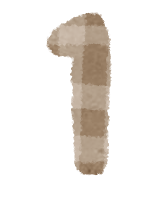
\includegraphics[keepaspectratio, scale=0.4]{number_1.png}
		\end{figure}
\end{document}
